\documentclass[border=8pt]{standalone}
\usepackage{tikz}
\usetikzlibrary{positioning,shapes.geometric,arrows.meta,calc,backgrounds,fit}

\definecolor{cnncolor}{RGB}{100,149,237}      % Cornflower blue - CNN layers
\definecolor{lstmcolor}{RGB}{255,165,0}       % Orange - LSTM layers
\definecolor{attncolor}{RGB}{220,20,60}       % Crimson - Attention
\definecolor{fusioncolor}{RGB}{60,179,113}    % Medium sea green - Fusion
\definecolor{fccolor}{RGB}{138,43,226}        % Blue violet - FC layers

\begin{document}
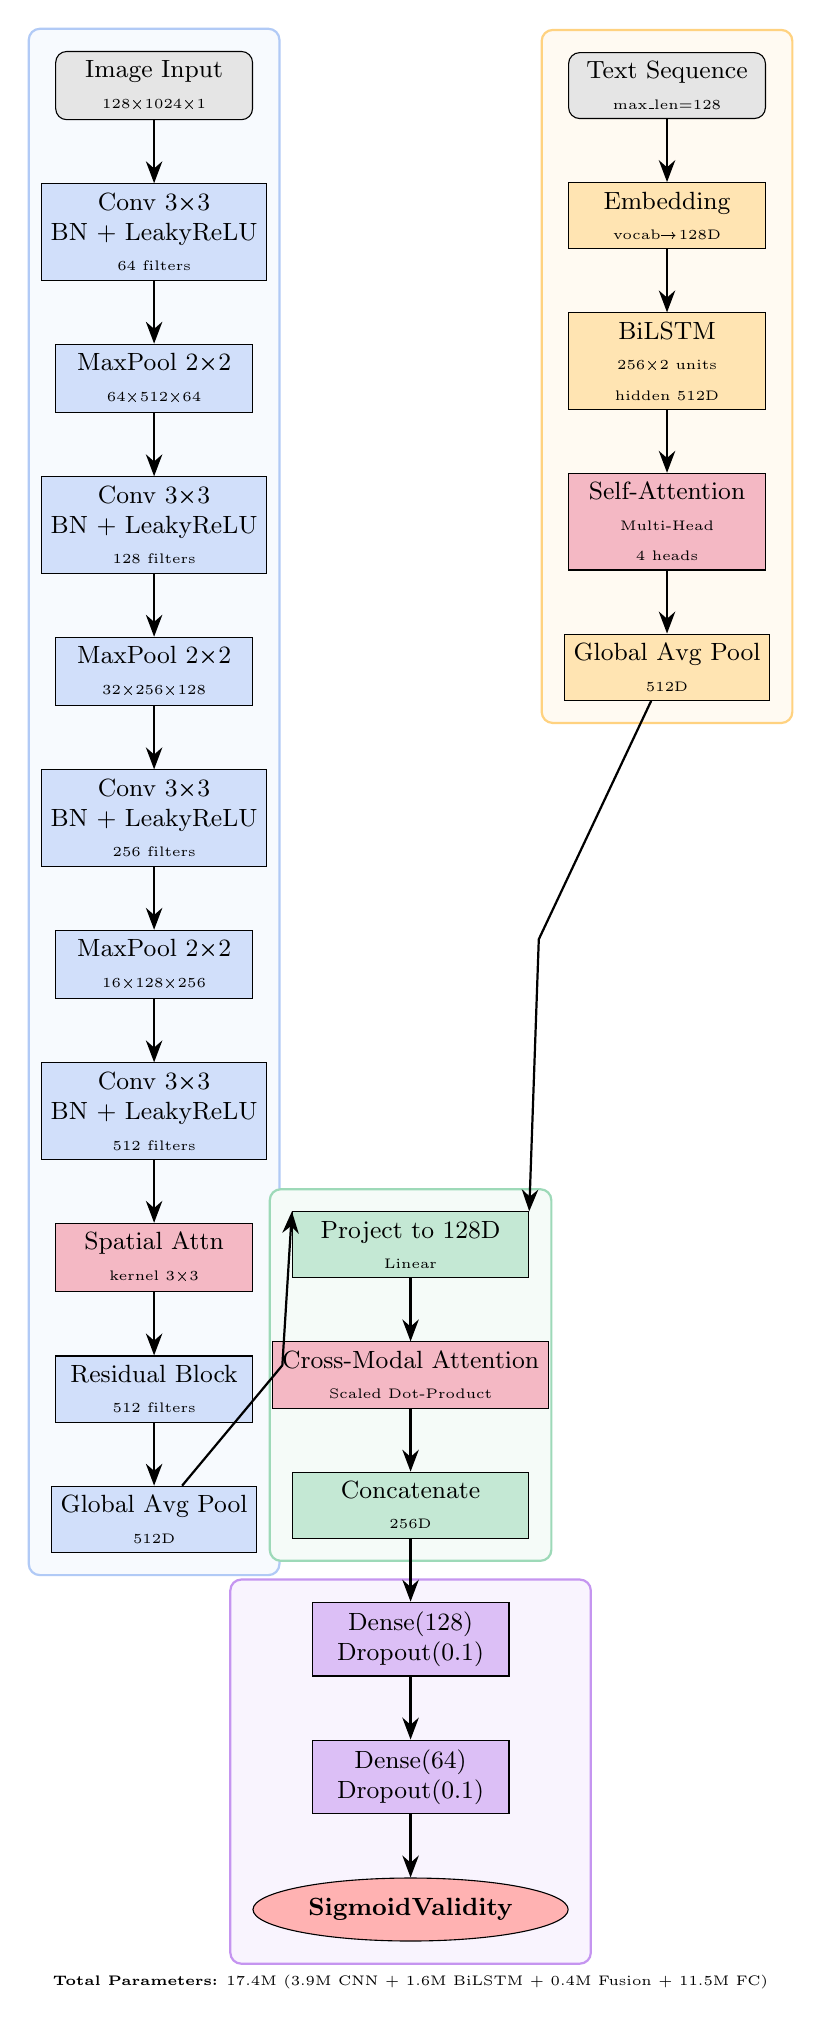
\begin{tikzpicture}[
    node distance=0.8cm,
    layer/.style={rectangle, draw, minimum width=2.5cm, minimum height=0.7cm, align=center, font=\small},
    cnn/.style={layer, fill=cnncolor!30},
    lstm/.style={layer, fill=lstmcolor!30},
    attn/.style={layer, fill=attncolor!30},
    fusion/.style={layer, fill=fusioncolor!30, minimum width=3cm},
    fc/.style={layer, fill=fccolor!30},
    input/.style={layer, fill=gray!20, rounded corners},
    output/.style={ellipse, draw, fill=red!30, minimum width=2.2cm, minimum height=0.8cm, font=\small\bfseries},
    arrow/.style={-{Stealth[scale=1.2]}, thick},
    skip/.style={-{Stealth[scale=1.2]}, thick, dashed, gray},
    label/.style={font=\tiny, align=center}
]

% ===== IMAGE BRANCH (LEFT) =====
\node[input] (img_in) at (0,0) {Image Input\\{\tiny 128×1024×1}};

\node[cnn, below=of img_in] (conv1) {Conv 3×3\\BN + LeakyReLU\\{\tiny 64 filters}};
\node[cnn, below=of conv1] (pool1) {MaxPool 2×2\\{\tiny 64×512×64}};

\node[cnn, below=of pool1] (conv2) {Conv 3×3\\BN + LeakyReLU\\{\tiny 128 filters}};
\node[cnn, below=of conv2] (pool2) {MaxPool 2×2\\{\tiny 32×256×128}};

\node[cnn, below=of pool2] (conv3) {Conv 3×3\\BN + LeakyReLU\\{\tiny 256 filters}};
\node[cnn, below=of conv3] (pool3) {MaxPool 2×2\\{\tiny 16×128×256}};

\node[cnn, below=of pool3] (conv4) {Conv 3×3\\BN + LeakyReLU\\{\tiny 512 filters}};
\node[attn, below=of conv4] (spatial_attn) {Spatial Attn\\{\tiny kernel 3×3}};
\node[cnn, below=of spatial_attn] (res_block) {Residual Block\\{\tiny 512 filters}};
\node[cnn, below=of res_block] (gap_img) {Global Avg Pool\\{\tiny 512D}};

% ===== TEXT BRANCH (RIGHT) =====
\node[input, right=4cm of img_in] (text_in) {Text Sequence\\{\tiny max\_len=128}};

\node[lstm, below=of text_in] (embed) {Embedding\\{\tiny vocab→128D}};
\node[lstm, below=of embed] (bilstm) {BiLSTM\\{\tiny 256×2 units}\\{\tiny hidden 512D}};
\node[attn, below=of bilstm] (self_attn) {Self-Attention\\{\tiny Multi-Head}\\{\tiny 4 heads}};
\node[lstm, below=of self_attn] (gap_text) {Global Avg Pool\\{\tiny 512D}};

% Align with image branch
\coordinate (align_point) at ($(gap_img)!0.5!(gap_text)$);

% ===== CROSS-MODAL FUSION =====
\node[fusion, below=1.5cm of align_point] (proj) {Project to 128D\\{\tiny Linear}};
\node[attn, below=of proj] (cross_attn) {Cross-Modal Attention\\{\tiny Scaled Dot-Product}};
\node[fusion, below=of cross_attn] (concat) {Concatenate\\{\tiny 256D}};

% ===== CLASSIFICATION HEAD =====
\node[fc, below=of concat] (fc1) {Dense(128)\\Dropout(0.1)};
\node[fc, below=of fc1] (fc2) {Dense(64)\\Dropout(0.1)};
\node[output, below=of fc2] (out) {Sigmoid\\Validity};

% ===== ARROWS - IMAGE BRANCH =====
\draw[arrow] (img_in) -- (conv1);
\draw[arrow] (conv1) -- (pool1);
\draw[arrow] (pool1) -- (conv2);
\draw[arrow] (conv2) -- (pool2);
\draw[arrow] (pool2) -- (conv3);
\draw[arrow] (conv3) -- (pool3);
\draw[arrow] (pool3) -- (conv4);
\draw[arrow] (conv4) -- (spatial_attn);
\draw[arrow] (spatial_attn) -- (res_block);
\draw[arrow] (res_block) -- (gap_img);

% ===== ARROWS - TEXT BRANCH =====
\draw[arrow] (text_in) -- (embed);
\draw[arrow] (embed) -- (bilstm);
\draw[arrow] (bilstm) -- (self_attn);
\draw[arrow] (self_attn) -- (gap_text);

% ===== ARROWS - FUSION =====
\draw[arrow] (gap_img) -- ($(gap_img)!0.5!(proj.north)$) -- (proj.north west);
\draw[arrow] (gap_text) -- ($(gap_text)!0.5!(proj.north)$) -- (proj.north east);
\draw[arrow] (proj) -- (cross_attn);
\draw[arrow] (cross_attn) -- (concat);
\draw[arrow] (concat) -- (fc1);
\draw[arrow] (fc1) -- (fc2);
\draw[arrow] (fc2) -- (out);

% ===== BACKGROUND GROUPS =====
\begin{pgfonlayer}{background}
    \node[draw=cnncolor!50, fill=cnncolor!5, rounded corners, thick, fit=(img_in)(gap_img), inner sep=8pt, label={[font=\footnotesize\bfseries, text=cnncolor]above:IMAGE BRANCH (CNN)}] {};
    
    \node[draw=lstmcolor!50, fill=lstmcolor!5, rounded corners, thick, fit=(text_in)(gap_text), inner sep=8pt, label={[font=\footnotesize\bfseries, text=lstmcolor]above:TEXT BRANCH (BiLSTM)}] {};
    
    \node[draw=fusioncolor!50, fill=fusioncolor!5, rounded corners, thick, fit=(proj)(concat), inner sep=8pt, label={[font=\footnotesize\bfseries, text=fusioncolor]above:CROSS-MODAL FUSION}] {};
    
    \node[draw=fccolor!50, fill=fccolor!5, rounded corners, thick, fit=(fc1)(out), inner sep=8pt, label={[font=\footnotesize\bfseries, text=fccolor]above:CLASSIFICATION}] {};
\end{pgfonlayer}

% ===== PARAMETER COUNT ANNOTATION =====
\node[label, below=0.3cm of out] {\textbf{Total Parameters:} 17.4M (3.9M CNN + 1.6M BiLSTM + 0.4M Fusion + 11.5M FC)};

\end{tikzpicture}
\end{document}
